\documentclass{article}
\usepackage{amsmath, amssymb, amsthm}
\usepackage{tikz}
\usetikzlibrary{arrows,shapes,positioning,shadows,trees,3d,angles,quotes,calc}
\usepackage{geometry}
\usepackage{graphicx}
\usepackage{float}
\usepackage{listings}
\usepackage{color}
\usepackage{algorithm}
\usepackage{enumitem}
\usepackage{siunitx}
\usepackage{threeparttable}
\usepackage{tablefootnote}
\usepackage[framemethod=tikz]{mdframed}
\geometry{a4paper, scale=0.8}

\title{Mathematical Modeling of Shot Put Throwing}
\author{Ethan\ Goh\ (No. 20230616)\\\texttt{7086cmd@gmail}}
\date{\today}

\begin{document}
\maketitle
\section*{Abstract}
There are multiple impacts on the result of the Shot Put competition, e.g. the speed of the ball, the throwing degrees, height, etc. Different factors can cause different results. This article used the kinetic principle and the mathematics model in the 2017 Athletics World Championships Women's Shot Put Final which includes Strike Speed, Strike Height, Strike Height Relative to Body Height, Distance Beyond Toe, Strike Tilt, etc., and created a model which uses gradient descent algorithm to analyze key points on the result of the Shot Put competition.

\section*{Keywords} Shot Put Competition, Gradient Descent, Kinetic Trace, Mathematics Model

\newpage

\tableofcontents

\newpage

\section{Introduction}

The ideal routine of the throwing trace is a parabola (as projectile motion). However, the trace isn't a parabola because of the air residence.

Without air residence, the trace will be like in \ref{fig:ideal-trace}.

\begin{figure}[H]
    \centering
    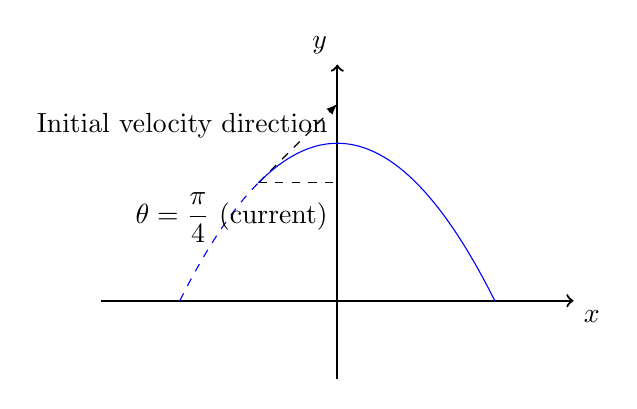
\begin{tikzpicture}
        \draw[thick, ->] (-3,0) -- (3,0) node[anchor=north west] {$x$};
        \draw[thick, ->] (0,-1) -- (0,3) node[anchor=south east] {$y$};
        \draw[scale=1,domain=-2:-1,dashed,smooth,variable=\x,blue] plot ({\x},{2-\x*\x/2});
        \draw[dashed, -latex] (-1, 1.5) -- (0, 2.5) node[anchor=north east] {Initial velocity direction};
        \draw[dashed] (-1, 1.5) -- (0, 1.5) node[anchor=north east] {$\theta=\dfrac{\pi}{4}$ (current)};
        \draw[scale=1,domain=-1:2,smooth,variable=\x,blue] plot ({\x},{2-\x*\x/2});
    \end{tikzpicture}
    \caption{Ideal trace}
    \label{fig:ideal-trace}
\end{figure}

However, because of the following reasons,

\begin{itemize}
    \item Air residence,
    \item Distortion of the throwing direction,
    \item Start position,
    \item $\dots$
\end{itemize}

The trace in \ref{fig:ideal-trace} is inaccurate.

Therefore, the article will develop a mathematical model for the trajectory of the shot put that includes the effect of air resistance. As for the distortion of the throwing direction, the article may use the 3D transforms with Euler angles to adjust the result.

\section{Parameters}

Some parameters are included, while some parameters are ignored.

\subsection{Parameters in Kinetic Model}

In the kinetic analysis, we don't bring the exact data. Some definitions are following the table \ref{table:parameters}.

\begin{table}[H]
    \centering
    \begin{threeparttable}
        \begin{tabular}{ccc}
            \hline
            \textbf{explain} & \textbf{parameter} & \textbf{e.g. value} \\
            \hline
            gravitational acceleration & $g$ & $9.787\si{\meter/\second^2}$ \\
            shot put mass & $m$ & $4\si{\kilo\gram}$ \\
            atmospheric drag coefficient & $k$ & N/A \\
            throw speed & $\boldsymbol{v}$ & N/A \tnote{1} \\
            throwing angle & $\theta$ & $37.0\si{\degree}$ \\
            throwing height & $h$ & $2.08\si{\meter}$ \\
            tilt angle left and right & $\varphi$ & $-21\si{\degree}$ \\
            horizontal displacement of the shot put \tnote{2} & $s$ & $19.94\si{\meter}$ \\
            \hline
        \end{tabular}
        \begin{tablenotes}
            \item [1] Actually, the speed is a vector, and the $v_x$, $v_y$ not only depend on the value of the absolute value but also on the throwing angle. Expressing with complex numbers is also OK, one of the examples is $13.24\mathrm{e}^{\cos37.0\si{\degree}+\mathrm{i}\sin37.0\si{\degree}}\si{\meter/\second}$, whose $v_y$ is $7.944\si{\meter/\second}$, and $v_x$ is $10.592\si{\meter/\second}$.
            \item [2] including exceeds toe board distance.
        \end{tablenotes}
    \end{threeparttable}
    \caption{Parameters of the Mathematical Model}
    \label{table:parameters}
\end{table}

We also assume the following conditions:

\begin{enumerate}
    \item The velocity is small, so $F=-kv$ should be used instead of $F=-kv^2$.
    \item The horizontal velocity is not reduced to $0$ due to air resistance.
    \item There is no influence of field forces other than the gravity field, which is assumed to be uniformly strong.
\end{enumerate}

\subsection{Parameters in the Regression Model}

\subsection{Ignore}

Because some parameters are useless, we ignore the following parameters:

\begin{enumerate}
    \item Front and rear tilt angles,
    \item Strike height relative to body height,
    \item Best round,
    \item \dots
\end{enumerate}

\section{Mathematical Model with Kinetic Analysis}

\label{section:mathematics-model}

\subsection{Force Analysis}

During the movement of a shot put ball, it is subjected to 2 forces: gravity and air resistance. The force of gravity is always vertically downward, however, air resistance changes with the direction of velocity.

The exciting thing is that we can break down air resistance in \ref{fig:force-situation}.

\begin{figure}[H]
    \centering
    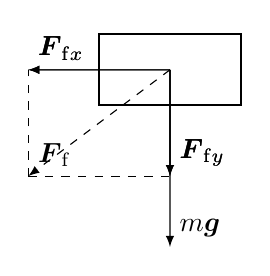
\begin{tikzpicture}[scale=1.8]
        \coordinate (A) at (0,0);
        \coordinate (B) at (1,0);
        \coordinate (C) at (1,0.5);
        \coordinate (D) at (0,0.5);
        \draw[thick] (A) -- (B) -- (C) -- (D) -- cycle;
        \coordinate (M) at (0.5,0.25);
        \draw[-latex] (M) -- (0.5,-1) node[anchor=south west] {$m\boldsymbol{g}$};
        \draw[-latex,dashed] (M) -- (-0.5,-0.5) node[anchor=south west] {$\boldsymbol{F}_\mathrm{f}$};
        \draw[-latex] (M) -- (0.5,-0.5) node[anchor=south west] {$\boldsymbol{F}_{\mathrm{f}y}$};
        \draw[-latex] (M) -- (-0.5,0.25) node[anchor=south west] {$\boldsymbol{F}_{\mathrm{f}x}$};
        \draw[-latex] (M) -- (0.5,-0.5) node[anchor=south west] {$\boldsymbol{F}_{\mathrm{f}y}$};
        \draw[-latex] (M) -- (-0.5,0.25) node[anchor=south west] {$\boldsymbol{F}_{\mathrm{f}x}$};
        \draw[dashed] (-0.5,-0.5) -- (0.5,-0.5);
        \draw[dashed] (-0.5,-0.5) -- (-0.5,0.25);
    \end{tikzpicture}
    \caption{Force Situation}
    \label{fig:force-situation}
\end{figure}

We define air resistance as $\boldsymbol{F}_\mathrm{f}=-k\boldsymbol{v}$. So, the residence vertically is $\boldsymbol{F}_{\mathrm{f}y}=-k\boldsymbol{v}_y$, and horizontal direction is the same.

\subsection{Vertical Motion}

There are 2 parts of the vertical motion, \textbf{ascend} and \textbf{descend}. However, we can regard them as a directed motion with the help of vectors.

\subsubsection{With Air Resistance}

Defining the direction vertically downward is the positive one, so $\boldsymbol{v}_0$, which is the primal velocity, is negative horizontally and vertically. Meanwhile, the acceleration of gravity, $g$, is positive vertically.

Via Newton's Second Theorem, we can know the force situation vertically:

\newcommand{\derive}{\mathrm{d}}

\begin{equation*}
    ma = mg - kv_y,
\end{equation*}

That is to say,

\begin{equation}
    m\dfrac{\derive v_y}{\derive t} = mg - kv_y
\end{equation}

Separate parametric variables and take integrals on both sides.

\begin{equation}
    \int\dfrac{\derive v_y}{mg - kv_y} = \int\dfrac{\derive t}{m}
\end{equation}

Then we can get

\begin{equation}
    -\dfrac{1}{k}\ln\left(mg-kv_y\right)=\dfrac{t}{m}+C
\end{equation}

Also bring in the initial velocity (vertical): $v_y\big\vert_{t=0}=v_0\sin\theta$ into the $C$, we can get the equation of vertical velocity:

\begin{equation}
    v_y=\dfrac{mg}{k}-\left(\dfrac{mg}{k}-v_0\sin\theta\right)\mathrm{e}^{-\frac{t}{m}k} \label{eq:vertical-velocity}
\end{equation}

Since we have defined the positive direction, we can simply integral the velocity to calculate the value of displacement:

\begin{equation}
    \int^t_0v_y\derive t=h
\end{equation}

We can solve this equation by methods such as Newton's method or Newton-like methods. After receiving $t$, we can get the horizontal displacement.

\subsubsection{Without Air Resistance}

If there is no air resistance, it is an ideal motion with gravity only. So the acceleration is simply $g$.

The motion time can be calculated with the height $h$:

\begin{equation}
    h = v_0\sin\theta t + \dfrac{1}{2}gt^2
\end{equation}

Then we can get the horizontal displacement after solving the equation whose result is $t$.

\subsection{Horizontal Motion}

The horizontal motion of the shot put is decelerated linear motion. However, the deceleration changes with the velocity.

\subsubsection{With Air Resistance}

Through Newton's Second Theorem, we can also get the horizontal force situation:

\begin{equation*}
    ma = kv_x
\end{equation*}

And the initial velocity (horizontal) is $v_0\cos\theta$. The methodology is consistent with the above, so it will not be repeated. After solving this differential equation, we can get the velocity:

\begin{equation}
    v_x=v_0\cos\theta\mathrm{e}^{-\frac{k}{m}t}
\end{equation}

Then we can use the integral to get the horizontal displacement.

\begin{equation}
    \int^t_0v_x\derive t=s
\end{equation}

It is important to note that since the magnitude of the air resistance is related to the velocity, differential equations must be used instead of the ordinary integral method. Since the equations in the vertical direction cannot be solved algebraically and directly, no simple and explicit algebraic relation among the parameters above can be given.

So, the trace of the shot put is in the figure \ref{fig:trace-with-residence}. That's a bit of an exaggeration.

\begin{figure}[H]
    \centering
    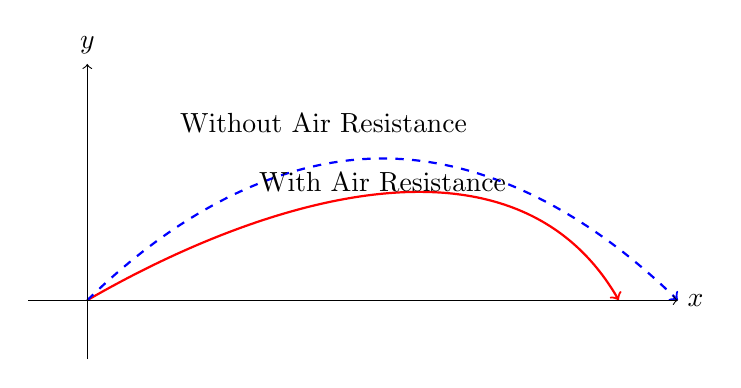
\begin{tikzpicture}[scale=1.5]
        \draw[thick,->,red] (0,0) to [out=30,in=120] (4.5,0);
        \draw[dashed, thick,->,blue] (0,0) parabola bend (2.5,1.2) (5,0);

        \node at (2,1.5) {Without Air Resistance};
        \node at (2.5,1) {With Air Resistance};

        \draw[->] (-0.5,0) -- (5,0) node[right] {$x$};
        \draw[->] (0,-0.5) -- (0,2) node[above] {$y$};

    \end{tikzpicture}
    \caption{The Trace of the Shot Put with Air Residence}
    \label{fig:trace-with-residence}
\end{figure}

\subsubsection{Without Air Resistance}

The horizontal motion without air resistance is a linear motion without any acceleration. When time is $t$, so the speed is $v_0\cos\theta$ all the time. So the displacement is:

\begin{equation}
    s=v_0\cos\theta t
\end{equation}

The full equation is used in the optimization, which doesn't consider the air resistance.

\section{Model Analysis}

The mathematical model uses differential equations to solve the question.

\subsection{Data Brought into the Analysis}

Using the formula \ref{eq:vertical-velocity}, we can get the vertical velocity of the shot put. Using \texttt{Geogebra}, we can get the $v_y-t$ graph in the figure \ref{fig:vy-t}. Data is used following the table \ref{table:parameters-data}.

\begin{table}[H]
  \centering
  \begin{threeparttable}
    \begin{tabular}{ccc}
      \hline
      \hspace{1cm}\textbf{Parameter}\hspace{1cm} & \hspace{1cm}\textbf{Value}\hspace{1cm} & \hspace{1cm}\textbf{Unit}\hspace{1cm} \\
      \hline
      $v_0$ & $-12$ & $\si{\meter/\second}$ \\
      $\theta$ & $37.0$ & $\si{\degree}$ \\
      $h$ & $2.08$ & $\si{\meter}$ \\
      $k$ & $0.00215$ \tnote{1} & $\si{\newton\cdot\second/\meter}$ \\
      $m$ & $4$ & $\si{\kilo\gram}$ \\
      \hline
    \end{tabular}
    \begin{tablenotes}
      \item [1] The value of $k$ is following the formula: $k=\dfrac{1}{2}C_DA\rho$, where $C_D$ is the drag coefficient, $A$ is the cross-sectional area, and $\rho$ is the air density. \\
      We regard the shot put as a sphere whose $r$ is $0.10 \si{\meter}$, and the air density is $1.225\si{\kilo\gram/\meter^3}$. So, the value of $k$ is $0.00215\si{\newton\cdot\second/\meter}$. \\
      The value of $k$ is not accurate, but it is enough for the model.
    \end{tablenotes}
  \end{threeparttable}
  \label{table:parameters-data}
  \caption{Parameters of the Mathematical Model}
\end{table}

\begin{figure}[H]
    \centering
    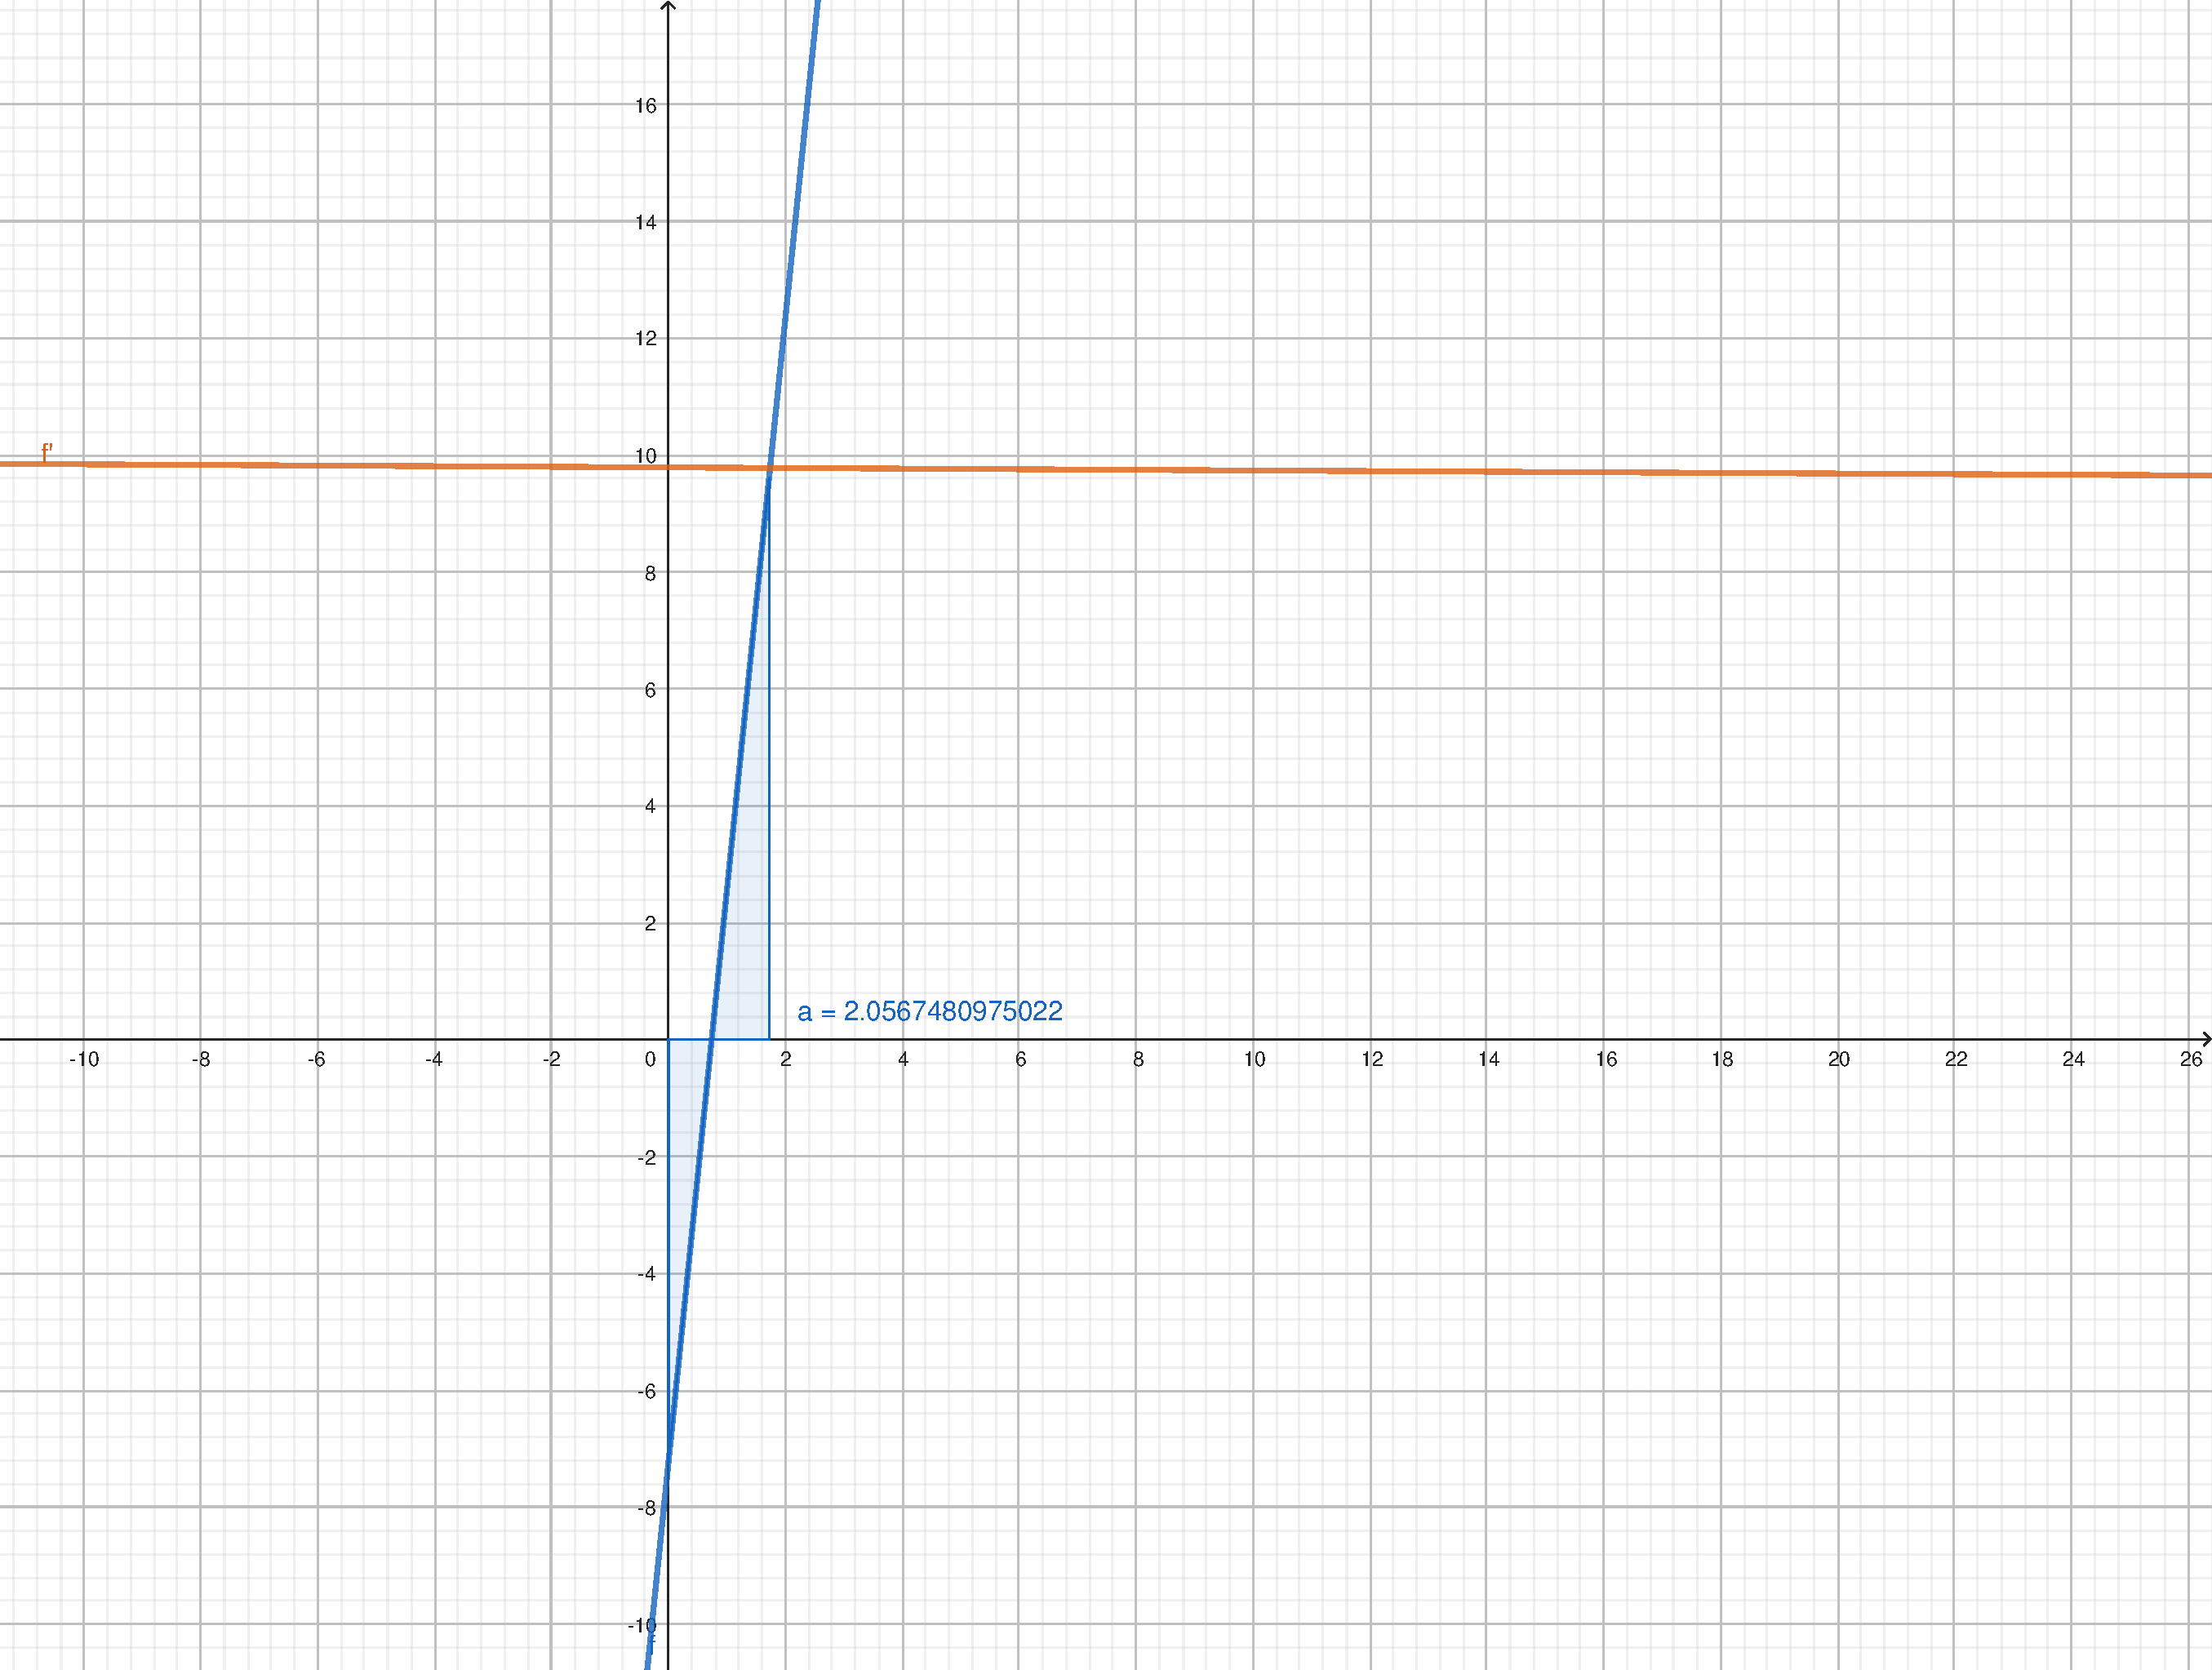
\includegraphics[width=0.6\textwidth]{figures/figure-1.pdf}
    \caption{The $v_y-t$ Graph}
    \label{fig:vy-t}
\end{figure}

The blue one is the graph, and the orange one is the derivative of the blue one. It seems that the velocity is decreasing little by little.

When $t \approx 1.76 \si{\second}$, the integral of the velocity, which is the displacement, is $2.08 \si{\meter}$, which is the throwing height.

Then, we can bring $t$ into the horizontal equation to get the horizontal displacement, which is the score.

\subsection{Example: Gong's Shot Put in 2017}

We selected Gong Lijiao's shot put in 2017 as an example. The data is in the attachment.

We set the $k = 0.00215$ and received the result of the horizontal displacement with the model, which returns $19.62599 \si{\meter}$, which is close to the real data.

Through \texttt{calculate/newton.py} provided in the attachment, we use \texttt{scipy} to calculate the approx value of $t$, which is $1.856988167816502 \si{\second}$.

Then we can get the horizontal displacement, which is $19.62599 \si{\meter}$, which is close to the real data ($1.6\%$ error).

If we add \textit{FB Truck Lean} into the release angle, the error will be reduced to $0.8\%$ ($19.78 \si{\meter}$).

\subsection{Features}

The mathematical model considers the air residence, which improves the accuracy of the model significantly. Ease of calculation through decomposition of motion.

\section{Optimization}

The optimization of the shot put can be implemented with the gradient descent method.

Because the air resistance is quite small, the solution of $t$ needs Newton's Method. So it is hard to implement the algorithm. In this part, we ignore the air resistance temporarily.

\subsection{Optimization Formula}

We regard impacts as the following:

\begin{enumerate}
    \item The initial velocity of the ball (negative because of its direction) $v$,
    \item The release angle $\theta$,
    \item The release height $h$,
    \item NOTE: Other related parameters (except distance) are not included in the model, we ignore them.
\end{enumerate}

The final formula of the optimization is the following:

\begin{equation}
    d = \dfrac{v_0\cos\theta\sqrt{v_0^2\sin^2\theta+2hg}-v_0\sin\theta}{g}
\end{equation}

We can use the gradient descent method to optimize the value of $v_0$, $\theta$, and $h$, to get the maximum value of $d$.

NOTE: The $d$ includes the distance beyond the toe board.

\subsection{Optimization Result}
\label{subsection:optimization-result}

We can get the optimization result through the code \texttt{optimize/grads.py} with the auto differentiation of \texttt{PyTorch}.

Be cautious that the optimization includes the limit, which is listed in the table \ref{table:optimization-result} (lower and upper limit depends on the absolute value):

\begin{table}[H]
    \centering
    \begin{tabular}{cccc}
        \hline
        \textbf{Parameter} & \textbf{Lower Limit} & \textbf{Upper Limit} & \textbf{Optimized Value} \\
        \hline
        $v_0$ & $-10.0\si{\meter/\second}$ & $-13.5\si{\meter/\second}$ & $13.5\si{\meter/\second}$ \\
        $\theta$ & $0\si{\degree}$ & $60.0\si{\degree}$ & $36.2\si{\degree}$ \\
        $h$ & $1.6\si{\meter}$ & $2.1\si{\meter}$ & $2.1\si{\meter}$ \\
        \hline
    \end{tabular}
    \caption{Optimization Result}
    \label{table:optimization-result}
\end{table}

And the result distance is $20.25\si{\meter}$.

It is easy to find out that the $h$ and the $v_0$ are the max in the range.

\subsection{Extra Ranges}

Except the $\theta$, $v_0$, and $h$ touch the max of the range. If the range is larger, the result will be different.

So we set the $h$ and $v_0$ bigger to see the result ($0.1$ each), and the result is following the table \ref{table:optimization-result-extend} (unit: \si{\meter}):


\begin{table}[H]
    \centering
    \begin{tabular}{ccccc}
        \hline
        \textbf{Parameter} & \textbf{Upper Result} & \textbf{Lower Result} & \textbf{Upper Diff} & \textbf{Lower Diff} \\
        \hline
        $h$ & $20.36\si{\meter}$ & $20.14\si{\meter}$ & $0.11\si{\meter}$ & $-0.11\si{\meter}$ \\
        $v_0$ & $20.52\si{\meter}$ & $19.99\si{\meter}$ & $0.27\si{\meter}$ & $-0.27\si{\meter}$ \\
        \hline
    \end{tabular}
    \caption{Optimization Result Extend}
    \label{table:optimization-result-extend}
\end{table}


It is easy to find out that the $v_0$ is more useful in this case.

\section{Evaluation}

This model uses the differential equation, gradient descent, etc. algorithms and successfully fits the real situation, which reduces the loss to about $1\%$ (distance). The air resistance is so tiny that we often ignore this factor, and it is subtle whether to use $f=-mv$ or $f=-mv^2$ in this situation.

\subsection{Advantages}

This model combines mathematics and computer technology which uses \texttt{PyTorch}, \texttt{scipy}, etc. that can reduce the calculation. We can get benefits from these techniques, which can automatically calculate the differential, and find the best value.

This module evaluated the impact of the tiny factor \textit{air resistance} which can be just ignored in the shot put competition for approx calculations.

The result of the model is good, which is $0.15\si{\meter}$ per line and $1\%$ among the full data.

\subsection{Disadvantages}

The model that used the differential equation needs to be solved with Newton's Method, which is hard to optimize. So the training of the target used the equation that doesn't include the air resistance and then brought the result into the equation that considers the air resistance. It's not very rigorous. Fortunately, we've proved that it is the optimal result in the near range, whether air resistance is considered.

The calculation of the model is complex so the author spent about 2 nights solving the differential equation. However, with the help of the computer, we can get the answer easily.

\section{Questions}

The modeling question raises several issues, and in this one section, the paper will present the introduction.

\subsection{Model Creating}

The mathematics model is introduced in \ref{section:mathematics-model}, and you can refer to the section to find the model. We used the data from the IAAF Championship which is contained in the attachments and bibliography part.

\subsection{Optimization}

The optimization result is declared in the section \ref{subsection:optimization-result}. It considered $v_0$, $h$, and $\theta$.

\section{Acknowledgement}

\begin{itemize}
    \item Thanks to the chance of the Zhenhai High School Math Festival Intramural Mathematical Modeling Competition, which provides the problem.
    \item Thanks to \texttt{PyTorch}, \texttt{scipy}, and other computing libraries so that I can calculate the result fast.
    \item Thanks to \LaTeX{} so that I can render my essay easily and conveniently.
    \item Thanks to \texttt{DeepL} and \texttt{Grammarly} so that I can modify my paper easily when there are some grammar mistakes.
    \item Thanks to my classmate Li Kangbo who referred the incompatibility of $f=-mv^2$ which doesn't reflects the alignment between $\boldsymbol{F}$ and $\boldsymbol{v}$ which is not capable to take the orthogonal decomposition.
\end{itemize}

\end{document}
